\documentclass[../Main.tex]{subfiles}
\begin{document}
  \chapter{2018-2019学年微积分（一）（下）期中考试}

  \section{基本计算题(每小题 6 分，共 60 分)}
  \begin{enumerate}
    \item 求微分方程$yy''+(y')^{2} = 0$满足初始条件$y(0)=1$，$y'(0)=\frac{1}{2}$的特解.
      \vspace{12em}

    \item 设$y=\mathrm{e}^{x}\left(C_{1}\sin 2x+C_{2}\cos 2x\right)$为某二阶常系数齐次微分方程的通解，求此微分方程.
      \vspace{12em}

    \item 已知点$A=(3,-3,1)$与点$B(3,-2,2)$满足$\overrightarrow{AM}= 3\overrightarrow
      {AB}$，求向量$\overrightarrow{OM}$的方向余弦.
      \vspace{12em}

    \item 判断直线$L_{1}:\frac{x+1}{2}=\frac{y-2}{-1}=\frac{z-4}{3}$与直线$L_{2}:
      \frac{x-1}{1}=\frac{y+3}{2}=\frac{z-6}{5}$是否共面.
      \vspace{13em}

    \item 讨论二重极限$\lim_{(x,y)\to (0,0)}\frac{x y^{2}}{x+y}$的存在性.
      若极限存在求其值，若不存在说明理由.
      \vspace{13em}

    \item 已知平面曲线由方程$x^{2}+y^{3}+\ln(x+y)-3=0$确定，求点$x=2,y=-1$处的法线方程.
      \vspace{14em}

    \item 设$\varphi(u,v)$有连续偏导数，方程$\varphi(cx-az,cy-bz)=0$确定隐函数$z=
      z(x,y)$. 证明：$az_{x}+bz_{y} = c$.
      \vspace{13em}

    \item 计算$I=\int_{0}^{2}\mathrm{d}y\int_{0}^{2}\max\left\{xy,1\right\}\mathrm{d}
      x$.
      \vspace{12em}

    \item 计算$I=\iint\limits_{D}\cos\left(x^{2}+y^{2}\right)\mathrm{d}x\mathrm{d}
      y$，其中$D=\left\{(x,y)|x^{2}+y^{2}\leq 4, |x|\geq |y|\right\}$.
      \vspace{12em}

    \item 计算$I=\iiint\limits_{V}\sqrt{x^{2}+y^{2}}\mathrm{d}x\mathrm{d}y\mathrm{d}
      z$，其中区域$V$由曲面$z=0,z=4-x^{2}-y^{2}$围成.
      \vspace{12em}
  \end{enumerate}

  \section{综合题(每小题 8 分，共 40 分)}
  \begin{enumerate}
    \setcounter{enumi}{10}

    \item 求解微分方程$y''-3y'+2y = \mathrm{e}^{2x}+\mathrm{e}^{3x}$.
      \vspace{12em}

    \item 求函数$u=2x+y^{2} z$在点$(1,-1,-1)$处沿椭球面$x^{2}+2y^{2}+3z^{2}=6$的外法线方向的方向导数.
      \vspace{11em}

    \item 求函数$u=x+3z$在曲线$\begin{cases}
        x+2y-3z=2,      \\
        x^{2}+y^{2} = 2
      \end{cases}$上的最大值与最小值.
      \vspace{11em}

    \item 求积分$I=\iiint\limits_{V}x^{2}\mathrm{d}x\mathrm{d}y\mathrm{d}z$，其中区域$V
      :x^{2}+y^{2}+z^{2}\leq 2z$.
      \vspace{11em}

    \item 设函数$f(x,y)=
      \begin{cases}
        \frac{xy^{3}}{x^{2}+y^{2}}, & (x,y)\neq (0,0), \\
        0,                          & (x,y)=(0,0).
      \end{cases}$

      （1）证明$f(x,y)$在$(0,0)$处可微；

      （2）求$f_{xy}(0,0)$.
      \vspace{11em}
  \end{enumerate}

  \chapter{2018-2019学年微积分（一）（下）期中考试参考答案}
  \section{基本计算题(每小题 6 分，共 60 分)}
  \begin{enumerate}
    \item \textbf{Solution}. 令$y'=p$，则$y''=\frac{\mathrm{d}p}{\mathrm{d}x}=\frac{\mathrm{d}p}{\mathrm{d}y}
      \cdot \frac{\mathrm{d}y}{\mathrm{d}x}= p\frac{\mathrm{d}p}{\mathrm{d}y}$，

      所以方程变形为$y p \cdot \frac{\mathrm{d}p}{\mathrm{d}y}+p^{2}=0$.

      显然$p\neq0$，故$y\frac{\mathrm{d}p}{\mathrm{d}y}+p=0$，即$y\mathrm{d}p + p
      \mathrm{d}y = \mathrm{d}(yp) = 0$.

      两边积分，得$yp = C_{1}$，将$y(0)=1$，$y'(0)=p(0)=\frac{1}{2}$代入上式，得$C
      _{1}= \frac{1}{2}$，所以$y\frac{\mathrm{d}y}{\mathrm{d}x}= \frac{1}{2}$，

      即$y\mathrm{d}y = \frac{1}{2}\mathrm{d}x$，两边积分，得$\frac{y^{2}}{2}= \frac{x}{2}
      + C_{2}$.

      将$y(0)=1$代入上式，得$C_{2}= \frac{1}{2}$，所以特解为$y= \sqrt{x+1}$.

    \item \textbf{Solution}. 由通解的形式可知特征方程的两个解为$1\pm 2i$，所以特征方程为$r
      ^{2}-2r+5=0$，

      因此二阶常系数齐次微分方程为$y''-2y'+5y=0$.

    \item \textbf{Solution}. 设$\overrightarrow{OM}= (x,y,z)$，则$\overrightarrow
      {AM}= (x-3,y+3,z-1)$，$\overrightarrow{AB}= (0,1,1)$.

      因$\overrightarrow{AM}= 3\overrightarrow{AB}$，所以$\begin{cases}
        x-3=0, \\
        y+3=3, \\
        z-1=3
      \end{cases}$，解得$\begin{cases}
        x=3, \\
        y=0, \\
        z=4.
      \end{cases}$

      故$\overrightarrow{OM}= (3,0,4)$，其方向余弦为$\cos \alpha = \frac{3}{5}$，$\cos
      \beta = 0$，$\cos \gamma = \frac{4}{5}$.

    \item \textbf{Solution}. 取$L_{1}$的方向向量$\boldsymbol{s}_{1} =(2,-1,3)$，$L
      _{2}$的方向向量$\boldsymbol{s}_{2} =(1,2,5)$，

      在$L_{1}$上取点$A(-1,2,4)$，在$L_{2}$上取点$B(1,-3,6)$，则$\overrightarrow{AB}
      = (2,-5,2)$. 计算

      $\overrightarrow{AB}\cdot \left(\boldsymbol{s}_{1} \times \boldsymbol{s}_{2}
      \right) =
      \begin{vmatrix}
        2 & -5 & 2 \\
        2 & -1 & 3 \\
        1 & 2  & 5
      \end{vmatrix}
      = 23\neq0$，所以$L_{1}$与$L_{2}$不共面.

    \item \textbf{Solution}. 因为$\lim_{\substack{(x,y)\to (0,0) \\ y = 0}}\frac{x
      y^{2}}{x+y}= 0$，

      $\lim_{\substack{(x,y)\to (0,0) \\ y=x^3-x}}\frac{x y^{2}}{x+y}= \lim_{x\to0}
      \frac{x(x^{3}-x)^{2}}{x+(x^{3}-x)}= \lim_{x\to0}\frac{x^{7}-2x^{5}+x^{3}}{x^{3}}
      =1$，

      因此$\lim_{\substack{x\to 0 \\ y\to 0}}\frac{x y^{2}}{x+y}$不存在.

      二重极限存在性问题，分母为$x+y$，常设$y = x^{\alpha}- x$来寻找不为0的极限值.

      再考虑一例：证明极限$\lim_{\substack{x\to 0 \\ y\to 0}}\frac{x^{3}y+xy^{4}+x^{2}y}{x+y}$不存在.

      \textbf{Solution}. 当$y=0$时，$\lim_{\substack{x\to 0 \\ y\to 0}}\frac{x^{3}y+xy^{4}+x^{2}y}{x+y}
      = 0$；

      令$y = x^{\alpha}- x$，$\frac{x^{3}y+xy^{4}+x^{2}y}{x+y}= \frac{x^{\alpha
      + 3}-x^{4}+x^{\alpha + 2}-x^{3}+x\left(x^{\alpha}-x\right)^{4}}{x^{\alpha}}
      = \frac{-x^{3} + o(x^{3})}{x^{\alpha}}$，

      令$\alpha = 3$，则$\lim_{\substack{(x,y)\to (0,0) \\ y = x^3-x}}\frac{x^{3}y+xy^{4}+x^{2}y}{x+y}
      = -1$，因此$\lim_{\substack{x\to 0 \\ y\to 0}}\frac{x^{3}y+xy^{4}+x^{2}y}{x+y}$不存在.

    \item \textbf{Solution}. 设$F(x,y) = x^{2}+y^{3}+\ln(x+y)-3$，

      曲线在点$(2,-1)$处的切线斜率$k = -\frac{F_{x}(2,-1)}{F_{y}(2,-1)}= - \left.
      \frac{2x+\frac{1}{x+y}}{3y^{2}+\frac{1}{x+y}}\right|_{(2,-1)}= -\frac{5}{4}$，所以法线斜率为$\frac{4}{5}$，

      因此法线方程为$y+1 = \frac{4}{5}(x-2)$，即$4x-5y-13=0$.

    \item \textbf{Solution}. 方程$\varphi(cx-az,cy-bz)=0$两边对$x$求偏导，得
      \[
        \varphi_{u}(c-az_{x}) + \varphi_{v}(-bz_{x}) = 0.
      \]

      所以$z_{x} = \frac{c\varphi_{u}}{a\varphi_{u}+b\varphi_{v}}$.

      方程$\varphi(cx-az,cy-bz)=0$两边对$y$求偏导，得
      \[
        \varphi_{u}(-az_{y}) + \varphi_{v}(c-bz_{y}) = 0.
      \]

      所以$z_{y} = \frac{c\varphi_{v}}{a\varphi_{u}+b\varphi_{v}}$.

      故$az_{x}+bz_{y} = \frac{c(a\varphi_{u}+b\varphi_{v})}{a\varphi_{u}+b\varphi_{v}}
      = c$.

    \item \textbf{Solution}.

      \noindent
      \begin{minipage}[c]{0.6\textwidth}
        积分区域如图所示. 所以
        \[
          \begin{aligned}
            I = & \iint\limits_{D_1}\mathrm{d}x\mathrm{d}y + \iint\limits_{D_2}xy\mathrm{d}x\mathrm{d}y                                                                        \\
            =   & 1 + \int_{\frac{1}{2}}^{2}\frac{1}{x}\mathrm{d}x + \int_{\frac{1}{2}}^{2}\mathrm{d}x\int_{\frac{1}{x}}^{2}xy\mathrm{d}y                                      \\
            =   & 1 + \ln x\Big|_{\frac{1}{2}}^{2}+ \int_{\frac{1}{2}}^{2}x\left(2-\frac{1}{2x^2}\right)\mathrm{d}x                                                            \\
            =   & 1 + 2\ln 2 + \int_{\frac{1}{2}}^{2}\left(2x-\frac{1}{2x}\right)\mathrm{d}x = 1 + 2\ln 2 + \left.\left(x^{2}-\frac{1}{2}\ln x\right)\right|_{\frac{1}{2}}^{2} \\
            =   & 1 + 2\ln 2 + 4 -\frac{1}{4}- \frac{1}{2}\ln 2 -\frac{1}{2}\ln 2 = \frac{19}{4}+ \ln 2.
          \end{aligned}
        \]
      \end{minipage}
      \hfill %
      \begin{minipage}[c]{0.5\textwidth}
        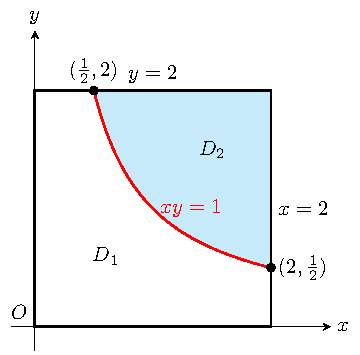
\includegraphics[width=6cm]{2019x-figure1.pdf} % 引入图片源
      \end{minipage}

    \item \textbf{Solution}.

      \noindent
      \begin{minipage}[c]{0.6\textwidth}
        积分区域如图所示. 所以
        \[
          \begin{aligned}
            I = & 4\iint\limits_{D_1}\cos\left(x^{2}+y^{2}\right)\mathrm{d}x\mathrm{d}y       \\
            =   & 4\int_{0}^{\frac{\pi}{4}}\mathrm{d}\theta\int_{0}^{2}r\cos r^{2}\mathrm{d}r \\
            =   & \pi\cdot\left.\frac{1}{2}\sin r^{2}\right|_{0}^{2}= \frac{\pi}{2}\sin 4.
          \end{aligned}
        \]
      \end{minipage}
      \hfill %
      \begin{minipage}[c]{0.5\textwidth}
        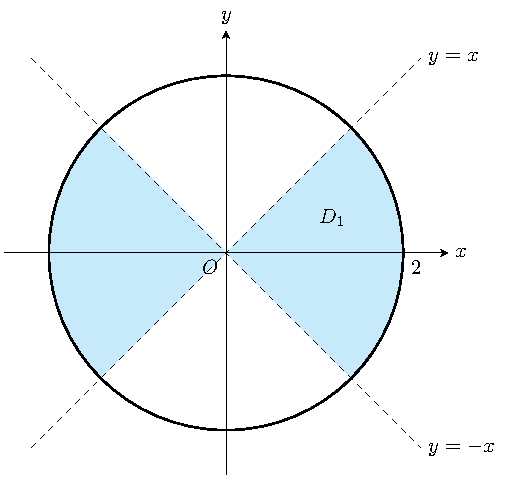
\includegraphics[width=5cm]{2019x-figure2.pdf} % 引入图片源
      \end{minipage}

    \item \textbf{Solution}. 用柱坐标代换，抛物面$z = 4 - x^{2} - y^{2}$可表示为$z
      = 4 - r^{2}$，所以

      \noindent
      \[
        \begin{aligned}
          I = & \iint\limits_{D}\mathrm{d}x\mathrm{d}y\int_{0}^{4-r^2}r\mathrm{d}z = \int_{0}^{2\pi}\mathrm{d}\theta\int_{0}^{2}r\mathrm{d}r\int_{0}^{4-r^2}r\mathrm{d}z \\
          =   & 2\pi\int_{0}^{2}r^{2}(4-r^{2})\mathrm{d}r = 2\pi\left.\left(\frac{4}{3}r^{3}-\frac{1}{5}r^{5}\right)\right|_{0}^{2}= \frac{128\pi}{15}.
        \end{aligned}
      \]
  \end{enumerate}

  \section{综合题(每小题 8 分，共 40 分)}
  \begin{enumerate}
    \setcounter{enumi}{10}

    \item \textbf{Solution}. 齐次方程$y''-3y'+2y = 0$的特征方程为$\lambda^{2}-3\lambda
      +2=0$，解得$\lambda = 1,2$，

      所以齐次方程的通解为$y = C_{1}\mathrm{e}^{x}+ C_{2}\mathrm{e}^{2x}$.

      分别求解非齐次项$\mathrm{e}^{2x}$和$\mathrm{e}^{3x}$对应的特解，

      对于$y_{1}=\mathrm{e}^{2x}$，$\lambda = 2$是齐次方程的特征根，所以可设特解为$y
      _{1}^{*}= Ax\mathrm{e}^{2x}$，

      将其代入$y''-3y'+2y = \mathrm{e}^{2x}$，得$4A\mathrm{e}^{2x}(1+x)-3A\mathrm{e}
      ^{2x}(1+2x)+2A x\mathrm{e}^{2x}= \mathrm{e}^{2x}$，

      解得$A = 1$，所以$y_{1}^{*}= x\mathrm{e}^{2x}$.

      对于$y_{2}=\mathrm{e}^{3x}$，$\lambda = 3$不是齐次方程的特征根，所以可设特解为$y
      _{2}^{*}= B\mathrm{e}^{3x}$，

      将其代入$y''-3y'+2y = \mathrm{e}^{3x}$，得$9B\mathrm{e}^{3x}-9B\mathrm{e}^{3x}
      +2B\mathrm{e}^{3x}= \mathrm{e}^{3x}$，

      解得$B = \frac{1}{2}$，所以$y_{2}^{*}= \frac{1}{2}\mathrm{e}^{3x}$.

      因此非齐次方程的通解为$y = C_{1}\mathrm{e}^{x}+ C_{2}\mathrm{e}^{2x}+ x\mathrm{e}
      ^{2x}+ \frac{1}{2}\mathrm{e}^{3x}$.

    \item \textbf{Solution}. 设$F(x,y,z) = x^{2}+2y^{2}+3z^{2}-6$，则$\nabla F(1,
      -1,-1) = (2, -4, -6)$，

      所以椭球面外法线方向的单位向量为$\boldsymbol{n}= \frac{1}{\sqrt{14}}(1, -2,
      -3)$.

      因此函数$u=2x+y^{2} z$在点$(1,-1,-1)$处沿椭球面$x^{2}+2y^{2}+3z^{2}=6$的外法线方向的方向导数

      $\frac{\partial u}{\partial \boldsymbol{n}}= \nabla u(1,-1,-1)\cdot \boldsymbol
      {n}= \frac{1}{\sqrt{14}}(2, 2, 1)\cdot (1, -2, -3) = -\frac{5\sqrt{14}}{14}$.

    \item \textbf{Solution}. 即在约束条件$\begin{cases}
        x+2y-3z = 2,    \\
        x^{2}+y^{2} = 2
      \end{cases}$下，求$x+3z$的最大值.

      用Lagrange乘数法，设$L(x,y,z,\lambda,\mu) = x+3z + \lambda\left(x+2y-3z-2\right
      ) + \mu\left(x^{2}+y^{2}-2\right)$，则

      \[
        \begin{cases}
          \frac{\partial L}{\partial x}= 1+\lambda + 2\mu x = 0 \\[6pt]
          \frac{\partial L}{\partial y}= 2\lambda + 2\mu y = 0, \\[6pt]
          \frac{\partial L}{\partial z}= 3 - 3\lambda = 0,      \\[6pt]
          \frac{\partial L}{\partial \lambda}= x+2y-3z-2 = 0,   \\[6pt]
          \frac{\partial L}{\partial \mu}= x^{2}+y^{2}-2 = 0.
        \end{cases}
      \]

      $\frac{\partial L}{\partial z}= 3 - 3\lambda = 0$，故$\lambda = 1$，将其代入$\frac{\partial
      L}{\partial x}= \frac{\partial L}{\partial y}= 0$，得$\mu x + 1 =\mu y + 1 =
      0$.

      所以$x=y$，代入$\frac{\partial L}{\partial \mu}= x^{2}+y^{2}-2 = 0$，得$x=y
      =1$或$x=y=-1$.

      当$x=y=1$时，$\frac{\partial L}{\partial \lambda}= x+2y-3z-2 = 0$，解得$z=\frac{1}{3}$，此时$x
      +3z = 2$；

      当$x=y=-1$时，$\frac{\partial L}{\partial \lambda}= x+2y-3z-2 = 0$，解得$z=
      -\frac{5}{3}$，此时$x+3z = -6$.

      因此函数$u=x+3z$在曲线$\begin{cases}
        x+2y-3z=2,      \\
        x^{2}+y^{2} = 2
      \end{cases}$上的最大值为$2$，最小值为$-6$.

    \item \textbf{Solution}. 用球坐标代换，球面$x^{2}+y^{2}+z^{2}\leq 2z$可表示为$r
      \leq 2\cos \varphi$，所以
      \[
        \begin{aligned}
          I = \iiint\limits_{V}x^{2}\mathrm{d}x\mathrm{d}y\mathrm{d}z = & \int_{0}^{2\pi}\mathrm{d}\theta\int_{0}^{\frac{\pi}{2}}\sin\varphi\mathrm{d}\varphi\int_{0}^{2\cos \varphi}r^{2}\cdot r^{2}\sin^{2}\varphi\cos^{2}\theta \mathrm{d}r \\
          =                                                             & \frac{32}{5}\int_{0}^{2\pi}\cos^{2}\theta\mathrm{d}\theta\int_{0}^{\frac{\pi}{2}}\sin^{3}\varphi\cos^{5}\varphi\mathrm{d}\varphi                                     \\
          =                                                             & \frac{32}{5}\cdot \pi\int_{0}^{\frac{\pi}{2}}\left(\cos^{2} \varphi - 1\right)\cos^{5} \varphi \mathrm{d}\cos\varphi                                                 \\
          =                                                             & \frac{32\pi}{5}\left.\left(\frac{1}{8}\cos^{8} \varphi - \frac{1}{6}\cos^{6} \varphi\right)\right|_{0}^{\frac{\pi}{2}}= \frac{4\pi}{15}.
        \end{aligned}
      \]

    \item \textbf{Solution}.

      （1）显然$f_{x}(0,0) = f_{y}(0,0) = 0$，

      所以即判断极限$\lim_{\substack{(x,y)\to (0,0)}}\frac{f(x,y)-f(0,0)-f_{x}(0,0)x-f_{y}(0,0)y}{\sqrt{x^{2}+y^{2}}}
      = \lim_{\substack{(x,y)\to (0,0)}}\frac{xy^{3}}{(x^{2}+y^{2})^{\frac{3}{2}}}$是否为$0$.

      因为$0 \leq \left|\frac{xy^{3}}{(x^{2}+y^{2})^{\frac{3}{2}}}\right| = \frac{|x|\cdot|y|^{3}}{(x^{2}+y^{2})^{\frac{3}{2}}}
      \leq \frac{|x|\cdot (x^{2}+y^{2})^{\frac{3}{2}}}{(x^{2}+y^{2})^{\frac{3}{2}}}
      = |x|$，且当$(x,y)\to (0,0)$时，$|x|\to 0$，

      由夹逼定理可知$\lim_{\substack{(x,y)\to (0,0)}}\frac{xy^{3}}{(x^{2}+y^{2})^{\frac{3}{2}}}
      = 0$，因此$f(x,y)$在$(0,0)$处可微.

      所以$\lim_{\substack{(x,y)\to (0,0)}}\frac{xy^{3}}{(x^{2}+y^{2})^{\frac{3}{2}}}
      = 0$，因此$f(x,y)$在$(0,0)$处可微.

      （2）$f_{x}(0,y)=\lim_{x\to0}\frac{f(x,y)-f(0,y)}{x}= \lim_{x\to0}\frac{y^{3}}{x^{2}+y^{2}}
      = y$，

      所以$f_{xy}(0,0) = \lim_{y\to0}\frac{f_{x}(0,y)-f_{x}(0,0)}{y}= \lim_{y\to0}
      \frac{y}{y}= 1$.
  \end{enumerate}
\end{document}
